\section{Resultados de la réplica v2}

Las 216 ejecuciones completaron 510 llamadas y 707,090 tokens. Se registraron 0 errores de infraestructura o protocolo. La contabilidad de todas las llamadas fue completa; los tokens no se estimaron. 

\subsection{Comparación principal: mismas tareas y modelo}

\begin{center}\small
\setlength{\tabcolsep}{4pt}
\begin{tabularx}{\linewidth}{@{}Xrrrrr@{}}
\toprule Configuración & Estricto & SQL norm. & Tokens & s/tarea & Llamadas \\ \midrule
Agente único & 19/24 & 23/24 & 1,160 & 4.62 & 24 \\
Secuencial & 20/24 & 24/24 & 3,343 & 12.47 & 72 \\
Paralela & 19/24 & 22/24 & 3,480 & 7.69 & 72 \\
Jerárquica & 18/24 & 22/24 & 4,532 & 11.13 & 96 \\
Reflexiva & 20/24 & 24/24 & 2,527 & 9.54 & 54 \\
SAGE-CREH & 23/24 & 23/24 & 1,765 & 7.34 & 38 \\
\bottomrule
\end{tabularx}\end{center}


Cada fila contiene 24 ejecuciones. Tokens y segundos son medias por tarea; llamadas es el total por condición. SQL norm. es una métrica secundaria de formato, no una reparación de respuestas.

\begin{center}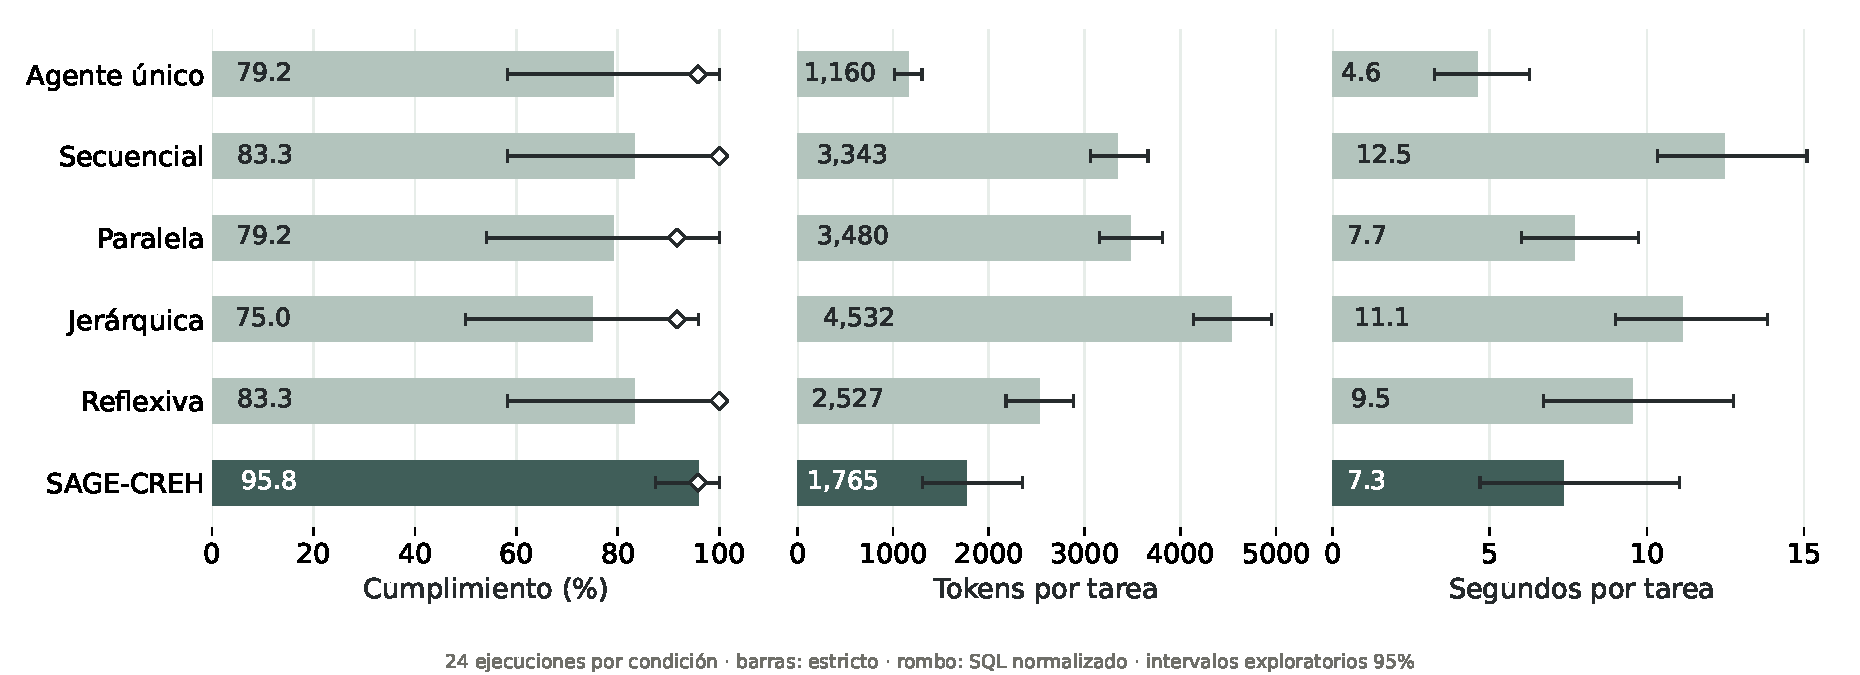
\includegraphics[width=\linewidth]{../../results/analysis-v2/comparison-es.pdf}\end{center}

Barras de cumplimiento estricto y marcas de SQL normalizado. Intervalos percentiles por tarea del 95\%; no prueban una clasificación general de arquitecturas.

\subsection{Cumplimiento por familia de tareas}

\begin{center}\small\begin{tabularx}{\linewidth}{@{}Xrrrrrr@{}}\toprule
Familia & Único & Sec. & Par. & Jer. & Refl. & SAGE \\ \midrule
Registros & 4 / 4 & 4 / 4 & 4 / 4 & 4 / 4 & 4 / 4 & 3 / 3 \\
Calendario & 3 / 3 & 4 / 4 & 4 / 4 & 2 / 2 & 4 / 4 & 4 / 4 \\
Dependencias & 4 / 4 & 4 / 4 & 2 / 2 & 4 / 4 & 4 / 4 & 4 / 4 \\
Selección & 4 / 4 & 4 / 4 & 4 / 4 & 4 / 4 & 4 / 4 & 4 / 4 \\
Memoria & 4 / 4 & 4 / 4 & 4 / 4 & 4 / 4 & 4 / 4 & 4 / 4 \\
SQL & 0 / 4 & 0 / 4 & 1 / 4 & 0 / 4 & 0 / 4 & 4 / 4 \\
\bottomrule\end{tabularx}\end{center}

Cada celda: aciertos estrictos / aciertos con SQL normalizado, ambos sobre cuatro ejecuciones de la familia (dos tareas por dos repeticiones). Fuera de SQL son la misma métrica.

\subsection{Controles de skills y delegación}

\begin{center}\small
\setlength{\tabcolsep}{4pt}
\begin{tabularx}{\linewidth}{@{}Xrrrrr@{}}
\toprule Configuración & Estricto & SQL norm. & Tokens & s/tarea & Llamadas \\ \midrule
Jerárquica & 18/24 & 22/24 & 4,532 & 11.13 & 96 \\
Jerárquica + 10 skills & 20/24 & 22/24 & 8,578 & 10.62 & 96 \\
SAGE-CREH & 23/24 & 23/24 & 1,765 & 7.34 & 38 \\
SAGE sin delegación & 21/24 & 21/24 & 1,110 & 5.93 & 24 \\
SAGE + 10 skills & 22/24 & 22/24 & 2,966 & 6.38 & 34 \\
\bottomrule
\end{tabularx}\end{center}


SAGE sin delegación conserva el proponente y las instrucciones de SAGE, eliminando solo el segundo resolutor y la revisión. SAGE con diez skills conserva la política, cambiando la carga de instrucciones. Los controles originales incluyen un catálogo de descripciones que SAGE no recibe; no atribuir toda diferencia a la topología.

\subsection{Diferencias emparejadas de consumo y tiempo}

\begin{center}\footnotesize\setlength{\tabcolsep}{3pt}\begin{tabularx}{\linewidth}{@{}Xrrrr@{}}\toprule
Comparación & Cambio tokens (\%) & IC 95\% & Diferencia s & IC 95\% \\ \midrule
Agente único & +52.2 & [15.9, 95.3] & +2.73 & [1.20, 4.97] \\
Secuencial & -47.2 & [-61.5, -29.5] & -5.13 & [-6.29, -3.77] \\
Paralela & -49.3 & [-62.3, -33.8] & -0.35 & [-1.73, 1.52] \\
Jerárquica & -61.1 & [-71.4, -48.5] & -3.79 & [-5.25, -2.30] \\
Reflexiva & -30.2 & [-51.8, -3.5] & -2.20 & [-5.33, 0.50] \\
SAGE sin delegación & +59.1 & [21.3, 99.0] & +1.42 & [0.46, 2.58] \\
SAGE + 10 skills & -40.5 & [-49.7, -29.6] & +0.96 & [-0.49, 2.94] \\
\bottomrule\end{tabularx}\end{center}

En cada fila: SAGE menos la configuración indicada; el cambio porcentual de tokens es 100(SAGE/control $-1$). Valores negativos favorecen menor consumo o tiempo de SAGE. Intervalos exploratorios de 10000 remuestreos emparejados por tarea.

\subsection{Rutas ejecutadas y efecto de las revisiones}

SAGE-CREH. Directa: 13; Acuerdo paralelo: 5; Arbitraje paralelo: 3; Revisión selectiva: 3. Frente al primer candidato: 5 correcciones y 0 regresiones de acierto estricto.

SAGE sin delegación. Directa: 24. Frente al primer candidato: 0 correcciones y 0 regresiones de acierto estricto.

SAGE + 10 skills. Directa: 15; Acuerdo paralelo: 7; Arbitraje paralelo: 1; Revisión selectiva: 1. Frente al primer candidato: 2 correcciones y 0 regresiones de acierto estricto.

Esta inspección usa el evaluador después de terminar las ejecuciones; nunca alimentó la política de enrutamiento. Una corrección puede ser de formato. Se conserva el detalle por ejecución.

\subsection{Desarrollo: resultados excluidos de la réplica}

Serial: 9/10; 1,606.7 tokens y 9.07 segundos medios.

Paralela: 10/10; 1,628.4 tokens y 8.11 segundos medios.

Se eligió la política paralela por mayor cumplimiento, según la regla previa. Desarrollo consumió 32,351 tokens en 28 llamadas y 20 ejecuciones. Este coste no se oculta en la réplica ni se suma a sus medias.

El único acierto que separó a los candidatos ocurrió en DEV22, de calendario: ambas políticas usaron la misma vía directa, sin riesgo ni revisión. La diferencia puede deberse a variación de generación y no demuestra una ventaja causal del paralelismo. Se conserva la elección conforme a la regla previa, sin reinterpretarla como prueba de superioridad.
